\documentclass[11pt,letterpaper]{book}

% Apress style packages
\usepackage[utf8]{inputenc}
\usepackage[T1]{fontenc}
\usepackage{lmodern}
\usepackage{geometry}
\geometry{letterpaper,margin=1in,top=1.25in,bottom=1.25in}

% Graphics and figures
\usepackage{graphicx}
\usepackage{float}
\usepackage{amssymb}
\graphicspath{{../images/}}

% Index
\usepackage{makeidx}
\makeindex

% Hyperlinks
\usepackage{hyperref}
\hypersetup{
    colorlinks=true,
    linkcolor=blue,
    filecolor=magenta,
    urlcolor=cyan,
    pdftitle={Introduction to Sora2},
    pdfauthor={Xu Zhiping},
}

% Chapter and section formatting
\usepackage{titlesec}
\titleformat{\chapter}[display]
  {\normalfont\huge\bfseries}{\chaptertitlename\ \thechapter}{20pt}{\Huge}
\titlespacing*{\chapter}{0pt}{0pt}{40pt}

% Custom commands for figure sizing
\newcommand{\figheight}{0.5\textheight}

% Captions
\usepackage{caption}
\captionsetup{font=small,labelfont=bf,justification=centering}

% Custom command for image copyright
\newcommand{\imgcopyright}[1]{\textit{\footnotesize #1}}
\newcommand{\authorcreated}{\imgcopyright{Generated by author using Sora2}}
\newcommand{\authorillustration}{\imgcopyright{Illustration by author}}

% Bibliography
\usepackage{natbib}
\bibliographystyle{apalike}

% Glossary
\usepackage[acronym]{glossaries}
\makeglossaries

% Load glossary definitions
% Glossary definitions for Sora2 book

% AI and Technical Terms
\newglossaryentry{sora2}{
    name=Sora2,
    description={OpenAI's advanced text-to-video generation system that converts natural language descriptions into dynamic video content}
}

\newglossaryentry{texttovideoGeneration}{
    name=Text-to-Video Generation,
    description={The process of creating video content from textual descriptions using artificial intelligence models}
}

\newglossaryentry{diffusionModel}{
    name=Diffusion Model,
    description={A type of generative model that learns to reverse a gradual noising process to generate new data samples}
}

\newglossaryentry{multimodalLearning}{
    name=Multimodal Learning,
    description={Machine learning approach that processes and integrates information from multiple modalities such as text, images, and video}
}

\newglossaryentry{promptEngineering}{
    name=Prompt Engineering,
    description={The practice of designing and optimizing text inputs to achieve desired outputs from AI systems}
}

% Filmmaking Terms
\newglossaryentry{cinematicLanguage}{
    name=Cinematic Language,
    description={The visual and auditory elements used in filmmaking to convey meaning, emotion, and narrative}
}

\newglossaryentry{visualGrammar}{
    name=Visual Grammar,
    description={The systematic rules and conventions that govern how visual elements combine to create meaning in moving images}
}

\newglossaryentry{shotComposition}{
    name=Shot Composition,
    description={The arrangement of visual elements within a frame to create aesthetic and narrative impact}
}

\newglossaryentry{emotionalArc}{
    name=Emotional Arc,
    description={The progression of emotional states throughout a narrative sequence, designed to engage and move the audience}
}

\newglossaryentry{storyboarding}{
    name=Storyboarding,
    description={The process of creating a sequence of drawings or images to pre-visualize a film or video sequence}
}

% Creative Process Terms
\newglossaryentry{iterativeRefinement}{
    name=Iterative Refinement,
    description={The process of gradually improving creative output through repeated cycles of generation, evaluation, and modification}
}

\newglossaryentry{secondLevelNarrative}{
    name=Second-Level Narrative,
    description={The art of creating complete emotional journeys within extremely compressed timeframes (2-15 seconds) using precise visual symbolism and psychological triggers}
}

\newglossaryentry{compressedStorytelling}{
    name=Compressed Storytelling,
    description={Narrative techniques that convey maximum emotional and narrative impact within minimal time constraints}
}

\newglossaryentry{visualSymbolism}{
    name=Visual Symbolism,
    description={The use of visual elements to represent ideas, emotions, or concepts beyond their literal meaning}
}

\newglossaryentry{rhythmSynchronization}{
    name=Rhythm Synchronization,
    description={The coordination of visual pacing with intended emotional beats and platform-specific attention patterns}
}

% Technical Workflow Terms
\newglossaryentry{humanAICollaboration}{
    name=Human-AI Collaboration,
    description={The cooperative process where human creativity and AI capabilities combine to produce enhanced creative outcomes}
}

\newglossaryentry{directorialLanguage}{
    name=Directorial Language,
    description={The specialized vocabulary and communication methods used to guide AI video generation systems toward specific creative visions}
}

\newglossaryentry{crossPlatformOptimization}{
    name=Cross-Platform Optimization,
    description={The practice of adapting content for optimal performance across different social media platforms and viewing contexts}
}

\newglossaryentry{ethicalAI}{
    name=Ethical AI,
    description={The responsible development and use of artificial intelligence systems with consideration for societal impact, bias, and transparency}
}

\newglossaryentry{realTimeGeneration}{
    name=Real-Time Generation,
    description={The capability to produce video content instantaneously or with minimal delay in response to user inputs}
}

% Acronyms
\newacronym{ai}{AI}{Artificial Intelligence}
\newacronym{ml}{ML}{Machine Learning}
\newacronym{gan}{GAN}{Generative Adversarial Network}
\newacronym{nlp}{NLP}{Natural Language Processing}
\newacronym{cv}{CV}{Computer Vision}
\newacronym{ui}{UI}{User Interface}
\newacronym{ux}{UX}{User Experience}
\newacronym{api}{API}{Application Programming Interface}
\newacronym{fps}{FPS}{Frames Per Second}
\newacronym{hd}{HD}{High Definition}
\newacronym{vr}{VR}{Virtual Reality}
\newacronym{ar}{AR}{Augmented Reality}
\newacronym{xr}{XR}{Extended Reality}

\begin{document}

\title{Chapter 1\\
\large Introduction to Sora2}
\author{Xu Zhiping\\
\small College of Computer Science and Artificial Intelligence\\
\small Fudan University}
\date{October 2025}
\maketitle

\tableofcontents

\setcounter{chapter}{0}
\chapter{Entering AI Video Generation: The Art of Turning Language into Light}
\label{ch:entering-ai-video}

\begin{chapterabstract}
This chapter introduces AI-powered text-to-video generation systems---exemplified by OpenAI's Sora 2 and Google's Veo 3---as revolutionary tools that transform natural language into dynamic visual content. Unlike traditional filmmaking tools, these platforms process linguistic inputs to generate complete cinematic sequences, making language the direct material of imagery. The chapter explores how AI video generators function as new visual grammar systems, interpreting subjects as compositions, verbs as camera movements, and adjectives as emotional filters. We examine the fundamental shift this technology represents: from industrial film production to accessible creative expression through natural language interface. The discussion covers dual-layer cognition---literal interpretation and emotional inference---demonstrating how these systems extract structured semantic signals from text to generate coherent visual narratives. While our primary examples focus on Sora 2, the principles apply equally to Veo 3 and emerging platforms. Through practical examples and theoretical frameworks, readers will understand how writing Prompts becomes a form of directorial action, enabling anyone to implement professional cinematographic techniques. This foundational chapter establishes the conceptual framework for mastering AI-powered filmmaking, preparing readers for the practical techniques explored in subsequent chapters.
\end{chapterabstract}

\section{Prologue: When Words Begin to Move}
\index{Sora 2!introduction}
\index{Veo 3!introduction}
\index{AI filmmaking!origins}

More than a century after the birth of cinema, humanity has welcomed another kind of ``camera''---one that requires neither lenses, film, nor crew. Platforms like OpenAI's Sora 2\index{Sora 2} and Google's Veo 3\index{Veo 3} are not cameras, nor are they special effects software; rather, they are \textbf{text-to-video generation systems that process natural language inputs}. They can transform a sentence, a poetic description, into a dynamic scene. Their revolutionary nature lies not in generating video, but in \textbf{making language the direct material of imagery}.

Imagine this: you type, ``At dawn, a cyclist crosses a bridge through the mist.'' Within seconds, the scene materializes: low-saturation cool tones, morning fog floating in humid air, the cyclist's breath turning white in the light. That atmosphere of solitude yet filled with hope requires no actors, cameras, or editing. With language alone, you can evoke sensation and emotion. The emergence of AI video generation means that writing no longer stops at ``words''---it becomes a form of ``directorial action.''

These AI platforms are not ordinary tools, but completely new \textbf{visual grammar systems}\index{visual grammar}. They process the layers and rhythms of language, transforming ``subjects'' into compositions, ``verbs'' into camera movements, and ``adjectives'' into color and light. Within Sora 2 and Veo 3's processing frameworks, ``a gentle breeze'' becomes a dynamic parameter, ``melancholy blue light'' becomes an emotional filter, and ``slow push-in shot'' becomes a temporal rhythm. What creators need to do is learn this new language---learn how to direct with words.

\section{Awakening of a New Medium: From Description to Direction}
\index{media evolution}
\index{creative revolution}

Every artistic revolution stems from the reinvention of expressive media \citep{manovich2001language}. The typewriter gave writers a sense of rhythm, the camera made painters reconsider light and shadow, and synthesizers allowed musicians to reshape melody. Now, Sora 2 brings ``imagery'' back to the embrace of words, becoming a \textbf{linguistic revolution in film}\index{linguistic revolution}. It makes ``writing shots'' possible, giving literary language the temporality and dynamism of cinema for the first time.

This transformation builds upon decades of research in generative models \citep{goodfellow2014generative} and multimodal machine learning, culminating in sophisticated text-to-video generation systems that can interpret natural language descriptions and translate them into coherent visual narratives \citep{singer2022make}.

In the world of Sora 2, verbs represent the curves of action, adjectives represent the emotional color palette, and nouns define composition and subject. For example:

\begin{Prompt}
``A young girl running in the rain, camera handheld following, light transitioning from cold blue to warm yellow.''
\end{Prompt}

As demonstrated in Figure \ref{fig:ch01-rain-running}, this Prompt generates a cinematic composition that effectively captures the emotional transition from melancholy to hope through color temperature and movement.

\begin{figure}[H]
\centering
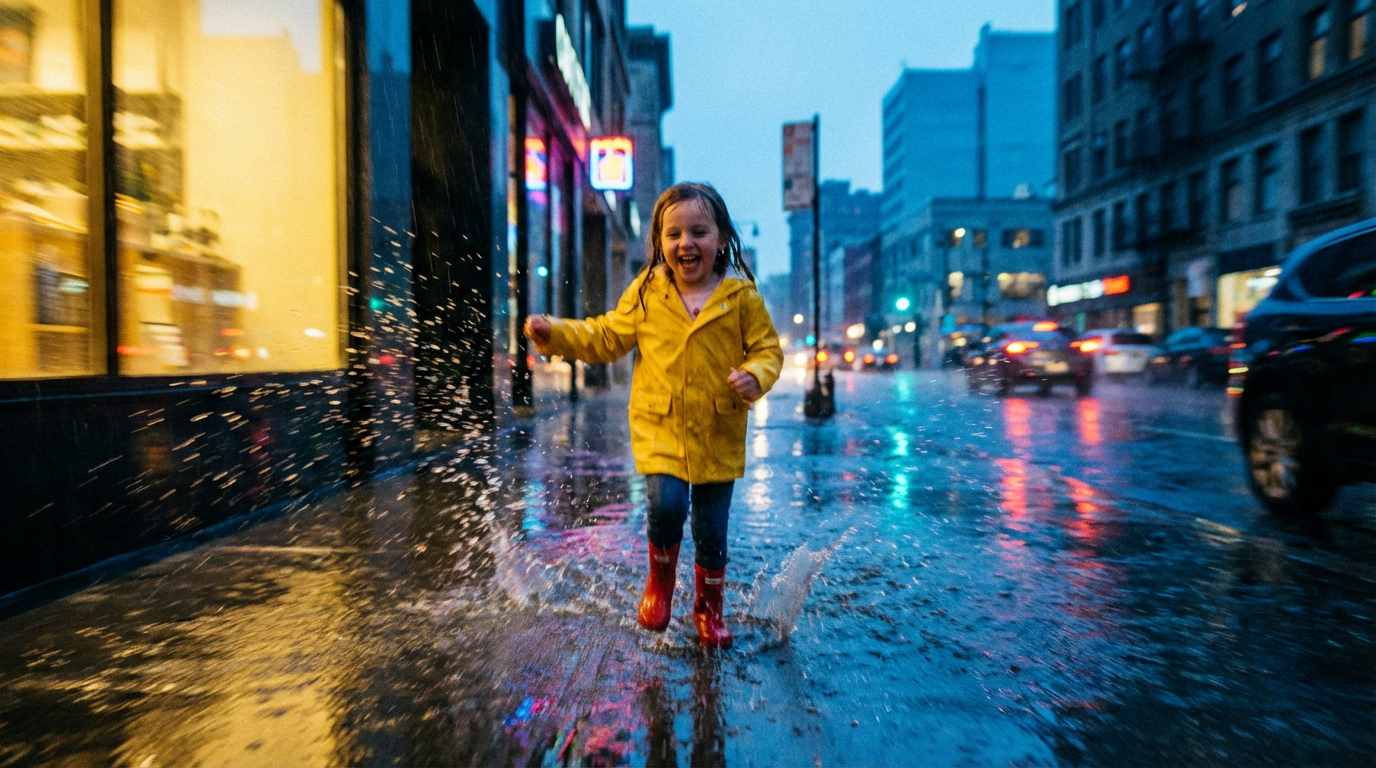
\includegraphics[height=\figheight]{Fig1-1.png}
\caption{Cinematic composition showing the transition from cold to warm tones \\ \authorcreated}
\label{fig:ch01-rain-running}
\end{figure}

This represents a complete \textbf{cinematographic instruction set}\index{cinematographic language}. Sora 2 interprets ``handheld'' as camera movement with natural shake and intimate framing, ``cold blue'' as color temperature indicating melancholic mood, and ``transitioning to warm yellow'' as a progressive emotional shift. The generated imagery demonstrates technical precision combined with emotional storytelling. Creators function as \textbf{visual directors using natural language}.

Sora 2 fundamentally changes the creator-audience relationship. Traditional cinema requires audiences to interpret directorial vision; Sora 2 enables everyone to directly implement cinematographic techniques. Film production shifts from industrial process to accessible creative tool. Users gain access to professional-level visual storytelling capabilities through natural language interface.

\section{Sora 2's Way of Thinking: Light and Rhythm in Semantics}
\index{semantic analysis}
\index{visual signals}

Sora 2 doesn't simply ``understand words.'' It analyzes language to generate \textbf{structured signals at the semantic level}. The system extracts five major dimensions from sentences: actions (verbs), objects (nouns), moods, settings, and camera intent. Each word becomes a trigger point for visual cues \citep{brooks2022instructpix2pix}.

When you input: ``On a rainy night street corner, flickering neon reflects a lonely silhouette.'' Sora 2 understands this is not a static image, but a visual poem with rhythm. It might choose slow motion, empty composition, and soft-focus halos, making loneliness ``flow'' visually. You are not just writing text; you are composing---using verbs to determine the beat, using adjectives to adjust harmony.

It possesses two layers of cognition:

\begin{itemize}
\item \textbf{Literal Layer}: Determines ``what to show''
\item \textbf{Lyrical Layer}\index{lyrical layer}: Determines ``how to show it''
\end{itemize}

This establishes Prompt writing as a technical discipline combining linguistic precision with visual design principles. Vocabulary specificity determines compositional elements; sentence rhythm influences camera movement patterns. Through practice, users develop \textbf{visual-linguistic thinking}---the ability to mentally preview shots while constructing Prompts.

\section{The ``Sora'' Concept: Accessibility and Creative Freedom}
\index{Sora!etymology}

``Sora'' means ``sky'' in Japanese, representing unlimited creative space and perspective. The name signifies \textbf{democratized access to professional filmmaking capabilities}. Sora 2 functions as a comprehensive visual production tool that removes traditional barriers to cinematic creation.

The system doesn't replace directors but expands directorial accessibility. Previously, complex aerial shots required significant budget and equipment; now, the same result is achievable through precise language: ``Camera moves through cloud layer, golden sunlight illuminating aircraft wing.'' Creative barriers shift from resource constraints to \textbf{linguistic precision and conceptual clarity}.

This accessibility transformation enables widespread creative participation. Language becomes the primary creative tool, emotion drives visual expression. Sora 2 shifts creative power from resource-dependent to skill-dependent, allowing poets, students, designers, and directors equal access to professional-quality visual storytelling.

\section{Prompt Literacy: Cultivating the Art from Text to Shot}
\index{Prompt literacy}
\index{creative training}

The real threshold of Sora 2 lies not in technology, but in \textbf{Prompt literacy}. This is the new Renaissance for 21st-century creators---an interdisciplinary cultivation from grammar to light and shadow. It requires creators to:

\begin{itemize}
\item Learn to ``write sentences with cinematographic thinking''
\item Understand the linguistic equivalents of editing rhythm and shot length
\item Embed emotional undercurrents in every short sentence
\end{itemize}

For example:

\begin{Prompt}
Basic Prompt: ``A person watching sunset by the sea.''

Advanced Prompt: ``Long shot following a man walking toward the seaside, orange sunset shattered into fragments by the waves, wind mixing with his calm breathing.''
\end{Prompt}

\begin{figure}[H]
\centering
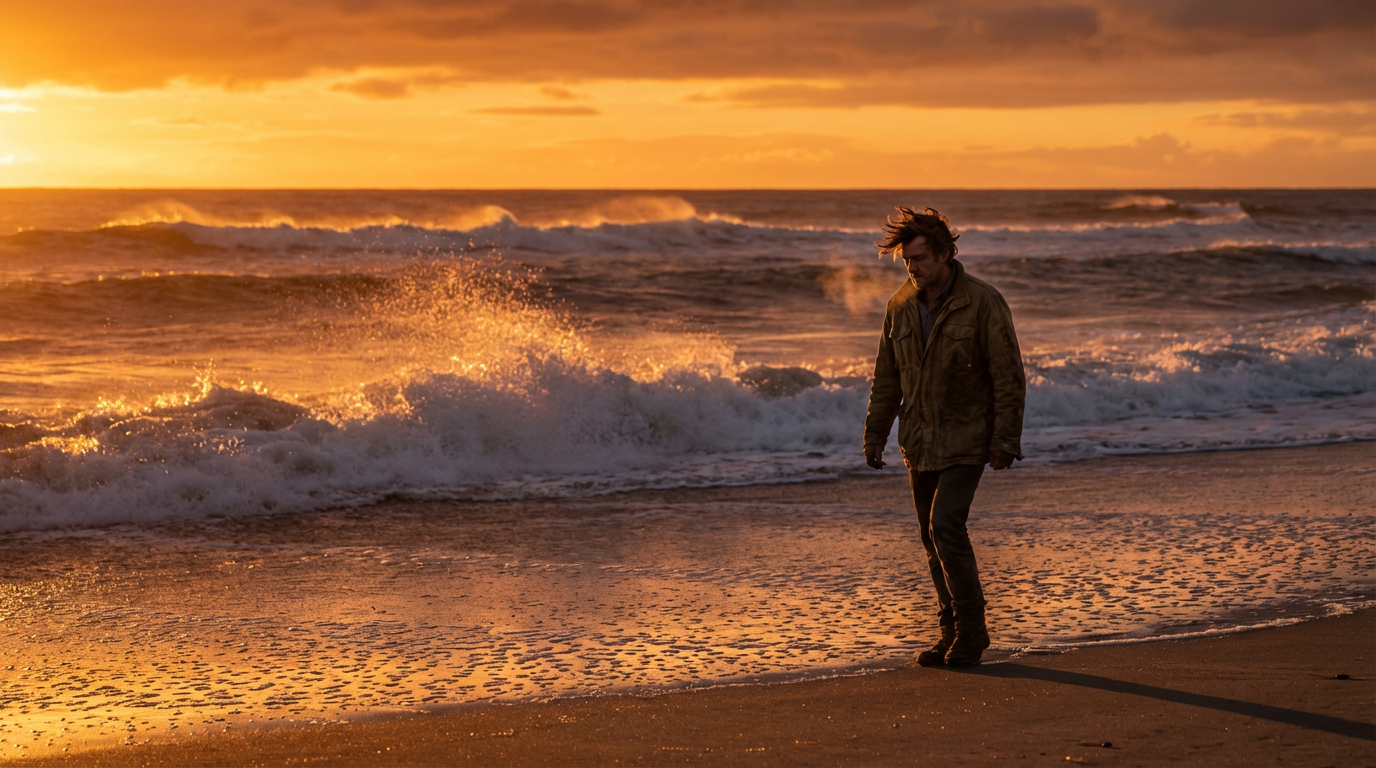
\includegraphics[height=\figheight]{Fig1-2.png}
\caption{Advanced cinematography: combining visual elements with emotional narrative \\ \authorillustration}
\label{fig:ch01-sunset}
\end{figure}

The advanced Prompt demonstrates superior visual composition and maintains narrative continuity through rhythm, composition, and emotional progression. Sora 2 interprets shot duration, lighting temperature, and atmospheric elements. The system functions beyond simple video generation---it \textbf{reconstructs experiential content}.

\section{Learning Progression: From Initial Use to Technical Mastery}
\index{learning curve}

User development typically follows three distinct phases:

\begin{enumerate}
\item \textbf{Discovery Phase}: Initial exposure to text-to-video transformation creates immediate recognition of the technology's potential.
\item \textbf{Calibration Phase}: Generated content may not match initial expectations, requiring understanding of AI interpretation patterns.
\item \textbf{Proficiency Phase}: Users develop systematic understanding of language-to-visual translation, enabling precise directorial control over AI output.
\end{enumerate}

These phases represent the technical learning progression for Sora 2 mastery. Effective collaboration requires understanding AI processing limitations and capabilities. Like professional directors working with actors, skilled Prompt writers must understand AI behavioral patterns and response mechanisms.

\section{Temporal Structure: Moment-Based Narrative Construction}
\index{narrative units}
\index{temporal rhythm}

Sora 2's fundamental narrative unit operates at the moment level rather than scene level. Each Prompt functions as a discrete temporal element within a larger rhythmic structure. Mastering this temporal precision enables complete story communication within seconds.

Example: ``She turns back with a smile, fireworks exploding behind her.'' This single sentence provides sufficient narrative information for cinematic climax construction. Sora 2 automatically applies appropriate temporal effects, lighting dynamics, and atmospheric synchronization. Effective creation prioritizes \textbf{selective moment amplification} over detail accumulation. This defines Sora-style narrative: concentrated storytelling, minimal shot requirements, maximum emotional impact.

\section{Technical Foundation: Understanding AI's Creative Capabilities}
\index{multimodal generation}
\index{text-to-video diffusion}

Sora 2's underlying architecture utilizes multimodal generative models (text-to-video diffusion). While technology provides the framework, effectiveness depends on \textbf{precise intention visualization}. The AI demonstrates advanced metaphorical interpretation capabilities---processing not only literal content but also emotional context.

Sora 2 functions as an artistic extension tool rather than replacement. It enables rapid experimentation across narrative formats: dreams, allegories, documentaries, advertisements, poetry. The system makes temporal storytelling techniques immediately accessible.

This represents a new creative instrument---responsive, efficient, and intuitive. It transforms conceptual ideas into visual form, enhances linguistic expression, and removes resource barriers from creative implementation.

\section{Implementation Framework: Collaborative Creation with Sora 2}
\index{co-creation}
\index{creative partnership}

Sora 2 operates as a collaborative creative tool rather than autonomous generator. It amplifies user inspiration through systematic emotion-to-vision translation. Each Prompt represents a communication protocol---users define visual parameters while the system provides technical interpretation and execution.

Future content creators will function as \textbf{cinematic language architects}. Sora 2 establishes the foundation for this evolution, restoring language-based creation and prioritizing conceptual clarity over resource availability.

\vspace{1em}
\hrule
\vspace{1em}

\section*{Practical Exercises}
\index{practical exercises}

\begin{quote}
\textit{\textbf{Timeless Principle:} Even as interfaces evolve and platforms update, the underlying visual logic---light, composition, rhythm, and emotional resonance---remains eternal. Master these fundamentals, and you will adapt effortlessly to any future tool.}
\end{quote}

\subsection*{Exercise 1: Basic Prompt Construction}
\textbf{Objective}: Learn to translate visual ideas into effective AI video Prompts (applicable to both Sora 2 and Veo 3).

\textbf{Task}: Transform these basic descriptions into cinematic Prompts:
\begin{enumerate}
\item "A person walking" → "A silhouetted figure walks slowly down a rain-soaked street, camera tracking from behind, warm streetlights creating golden reflections on wet pavement"
\item "A cat sleeping" → "Close-up of a tabby cat curled on a sunlit windowsill, soft focus background, gentle breathing rhythm, golden hour lighting"
\item "Someone cooking" → "Overhead shot of hands kneading dough, flour particles floating in morning light streaming through kitchen window, rhythmic movements"
\end{enumerate}

\subsection*{Exercise 2: Emotional Translation}
\textbf{Objective}: Practice converting emotions into visual language.

\textbf{Task}: Create Prompts that convey these emotions without explicitly naming them:
\begin{itemize}
\item Loneliness: "Single chair in empty café, rain streaking windows, muted colors, distant city sounds"
\item Hope: "Sunrise breaking through storm clouds, camera slowly rising, warm light gradually overtaking cool shadows"
\item Nostalgia: "Old photograph on wooden table, soft sepia tones, gentle breeze moving curtains, dust particles in afternoon light"
\end{itemize}

\subsection*{Exercise 3: Cross-Platform Prompt Testing}
\textbf{Objective}: Understand how the same Prompt performs across different AI video platforms.

\textbf{Task}: Use this universal Prompt on both Sora 2 and Veo 3 (if you have access to both):
\begin{Prompt}
"A musician plays piano in an empty concert hall, camera slowly circles, late afternoon light streaming through tall windows, dust particles floating in golden beams"
\end{Prompt}

\textbf{Compare and document}:
\begin{itemize}
\item Visual quality and lighting interpretation
\item Motion smoothness and camera movement execution
\item Audio presence (Veo 3 generates ambient sound; Sora 2 requires separate audio)
\item Generation time and overall fidelity to Prompt
\end{itemize}

This exercise demonstrates that strong Prompt writing skills transfer across platforms---the visual logic remains universal.

\section*{Prompt Templates}
\index{Prompt templates}

\subsection*{Template 1: Basic Scene Construction}
\begin{Prompt}
\textbf{[Subject]} + [Action] + [Setting] + [Lighting] + [Camera Movement] + [Mood/Atmosphere]

Example: "Young woman + reading book + cozy library corner + warm lamplight + slow zoom in + peaceful contemplation"
\end{Prompt}

\subsection*{Template 2: Cinematic Storytelling}
\begin{Prompt}
\textbf{[Establishing Shot]} → [Character Introduction] → [Emotional Beat] → [Visual Metaphor]

Example: "Wide shot of bustling city street → close-up of elderly man feeding pigeons → gentle smile as birds gather → camera pulls back revealing him as island of calm in urban chaos"
\end{Prompt}

\subsection*{Template 3: Atmospheric Mood Creation}
\begin{Prompt}
\textbf{[Time of Day]} + [Weather/Environment] + [Color Palette] + [Symbolic Elements] + [Emotional Undertone]

Example: "Golden hour + light mist + warm amber tones + floating dandelion seeds + bittersweet farewell"
\end{Prompt}

\section*{Quality Checklist}
\index{quality checklist}

\subsection*{Pre-Generation Checklist}
Before submitting your Prompt, verify:

\begin{itemize}
\item[$\square$] \textbf{Visual Clarity}: Can you clearly visualize the scene from your description?
\item[$\square$] \textbf{Cinematic Elements}: Have you included camera angle, movement, or framing?
\item[$\square$] \textbf{Lighting Description}: Is the lighting mood and quality specified?
\item[$\square$] \textbf{Emotional Intent}: Does the Prompt convey the intended feeling?
\item[$\square$] \textbf{Specificity Balance}: Detailed enough to guide, open enough for AI creativity?
\item[$\square$] \textbf{Technical Feasibility}: Are you requesting achievable visual elements?
\end{itemize}

\subsection*{Post-Generation Evaluation}
After reviewing generated content:

\begin{itemize}
\item[$\square$] \textbf{Narrative Coherence}: Does the visual tell a clear story?
\item[$\square$] \textbf{Emotional Resonance}: Does it evoke the intended feeling?
\item[$\square$] \textbf{Technical Quality}: Are lighting, composition, and movement satisfactory?
\item[$\square$] \textbf{Creative Surprise}: Did the AI add unexpected but valuable elements?
\item[$\square$] \textbf{Iteration Potential}: What could be refined in the next version?
\end{itemize}

\section*{Common Beginner Mistakes and Solutions}
\index{common mistakes}

\begin{table}[H]
\centering
\caption{Beginner Prompt Issues and Corrections \\ \authorillustration}
\label{tab:beginner-mistakes}
\begin{tabular}{p{4cm}p{4cm}p{5cm}}
\hline
\textbf{Common Mistake} & \textbf{Problem} & \textbf{Solution} \\
\hline
"A beautiful sunset" & Too vague, no direction & "Golden sunset through pine trees, camera slowly panning right, warm orange light filtering through branches" \\
\hline
"Person running very fast with lots of action and excitement" & Overloaded, unclear focus & "Runner in motion, camera tracking alongside, determined expression, rhythmic breathing visible in cold air" \\
\hline
"Make it look professional" & Non-visual instruction & "Shallow depth of field, cinematic color grading, stable camera movement, professional lighting setup" \\
\hline
"Like a movie scene" & Too generic & "Film noir style, dramatic shadows, single light source from window, black and white with selective color" \\
\hline
\end{tabular}
\end{table}

\section*{Chapter Summary}

Key actionable insights for entering AI video generation with Sora 2 and Veo 3:

\begin{itemize}
\item \textbf{Prompt Literacy}: Develop the skill to translate visual concepts into precise textual descriptions---this skill transfers across all AI video platforms
\item \textbf{Co-Creation Mindset}: Approach Sora 2 and Veo 3 as collaborative partners rather than automated tools
\item \textbf{Language-to-Light Translation}: Practice describing scenes with cinematic terminology (lighting, angles, movement)
\item \textbf{Platform Awareness}: Understand that Sora 2 excels in extended duration and Cameo features, while Veo 3 offers native audio generation
\item \textbf{Iterative Learning}: Start with simple Prompts and gradually increase complexity as you understand each system
\item \textbf{Creative Freedom}: Focus on imagination and storytelling rather than technical limitations---the principles remain constant across platforms
\end{itemize}

\begin{Prompt}
\textit{Writing is thinking with words; directing is thinking with images; and AI video generation is thinking about images with language.}
\end{Prompt}


\bibliography{../references}

\printindex

\end{document}
